% !TeX spellcheck = en_US
\documentclass[a3paper, 11pt]{article}
\usepackage{comment} % enables the use of multi-line comments (\ifx \fi) 
\usepackage{fullpage} % changes the margin
\usepackage{vhistory}
\usepackage{graphicx}
\usepackage{enumitem}

\newlength{\drop}
\newcommand\tab[1][1cm]{\hspace*{#1}}


\begin{document}
	
	\begin{titlepage}
		\drop=0.1\textheight
		\centering\vspace*{\baselineskip}
		\rule{\textwidth}{1.6pt}\vspace*{-\baselineskip}\vspace*{2pt}
		\rule{\textwidth}{0.4pt}\\[\baselineskip]
		{\LARGE \textbf{USER HANDBOOK \\ PROJECT 2 : 6502 Debugger}}\\[0.2\baselineskip]
		\rule{\textwidth}{0.4pt}\vspace*{-\baselineskip}\vspace{3.2pt}
		\rule{\textwidth}{1.6pt}\\[\baselineskip]
		\scshape
		\vspace*{2\baselineskip}
		Edited by \\[\baselineskip]
		{\Large Frazer Bayley \\ Haley Whitman \\ Abdulaziz Al-Heidous \\ Alison Legge \\ Jeremy Brennan\par}
		
		\vfill
		{\scshape \LARGE Project 2 -} \        {\LARGE Team 3}\par	
	\end{titlepage}

\tableofcontents

\vspace*{10\baselineskip}
\begin{versionhistory}
	\vhEntry{.1}{11.03.17}{Alison Legge}{Created initial outline of document}
\end{versionhistory}
\pagebreak	

\section{Introduction}
\subsection{The 6502 Debugger}
Thank you for using this 6502 Debugger. This 6502 Debugger is designed for a retro software developer who may have an interest in analyzing 6502 assembly code. It provides functionality such as the ability to assemble, execute, and step through code, and importing and exporting several different programs. 

\subsection{How to Use this Handbook}
This handbook covers a range of scenarios you might encounter when using this Debugger. This handbook will walk you through each scenario step-by-step.
\begin{itemize}
	\item \textbf{Read Every Step:}\\
	Make sure you do not skip any steps that are listed in this handbook. Every step has been carefully thought out to make using the Debugger easier. 
	\item \textbf{Use the Handbook in Conjunction with the 6502 Debugger:}\\
	After your first read through of the handbook, have it open and ready as you first start to use the 6502 Debugger. 
	\item \textbf{Experiencing Issues:}\\
	If you are experiencing issues and are unable to solve it with the help of this handbook, please contact our support team. 
\end{itemize}
\pagebreak

\section{Getting Started with the 6502 Debugger}
\subsection{Download and Install}
The development team will gave sent you the 6502-Debugger.jar file that launches the application. In case you did not receive the link or have lost the 6502-Debugger.jar file, contact the support team. 
\subsection{Starting the Application}
To launch the application, select and open the 6502-Debugger.jar file. This will immediately launch the Debugger application. If you have any problems, please contact the support team. Enjoy!
\pagebreak

\section{Importing Assembly Code}
\subsection{Overview}
Importing assembly code is easy to do with this 6502 Debugger, just make sure you are using 6502 ISA assembly code.
\subsection{Procedure}
\begin{enumerate}
	\item \textbf{Begin at the Main Page}\\
	Below is an image of the main page to help you verify you are where you need to be.
	\begin{figure}[h!]
		\centering
			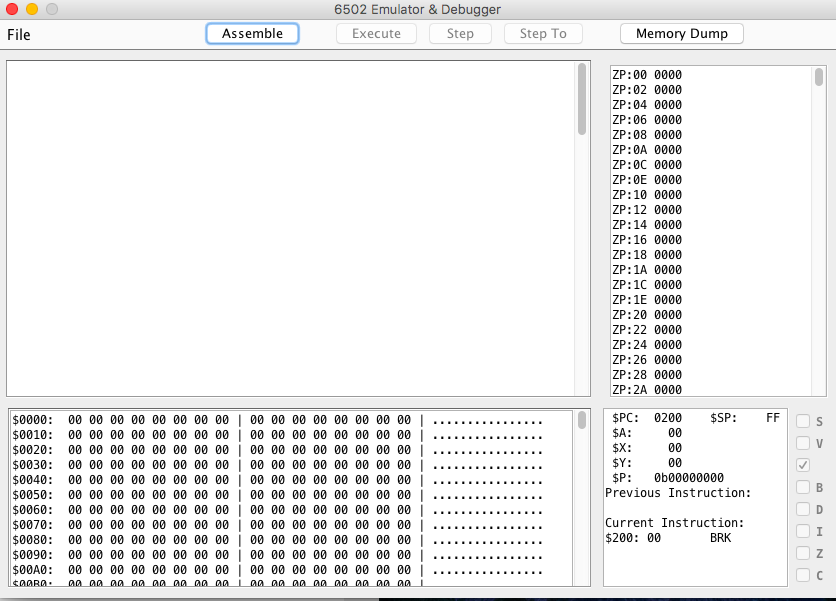
\includegraphics[width=9cm, height=6.4cm]{MainPage}
			\caption{Main Page}
	\end{figure}
	\clearpage
	\item \textbf{Click Open in the drop down File Menu}
	You will see the File menu on the top left-hand corner of the window. Click File so the drop down menu appears and click Open, a new window will appear. 
	\begin{figure}[h!]
		\centering
			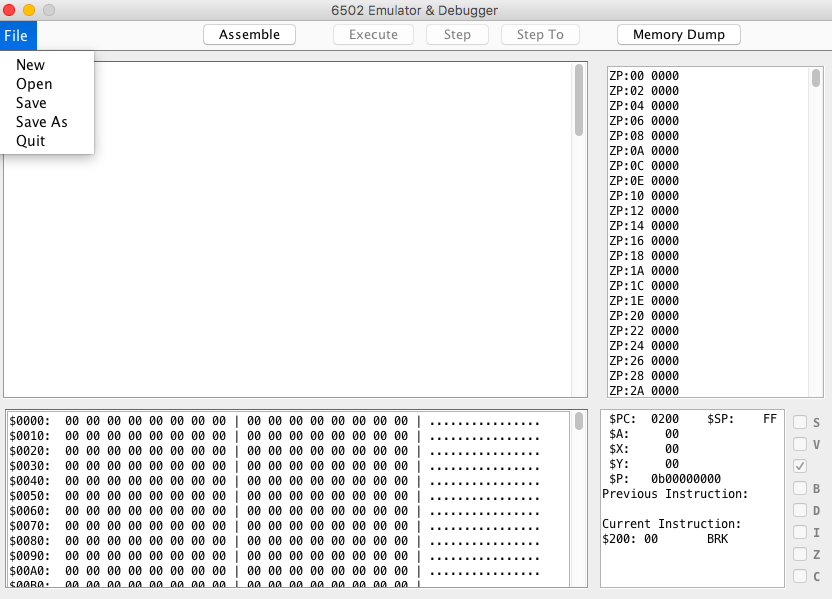
\includegraphics[width=9cm, height=6.4cm]{FileMenu}
			\caption{Drop down File Menu}
	\end{figure}
	\begin{figure}[h!]
		\centering
		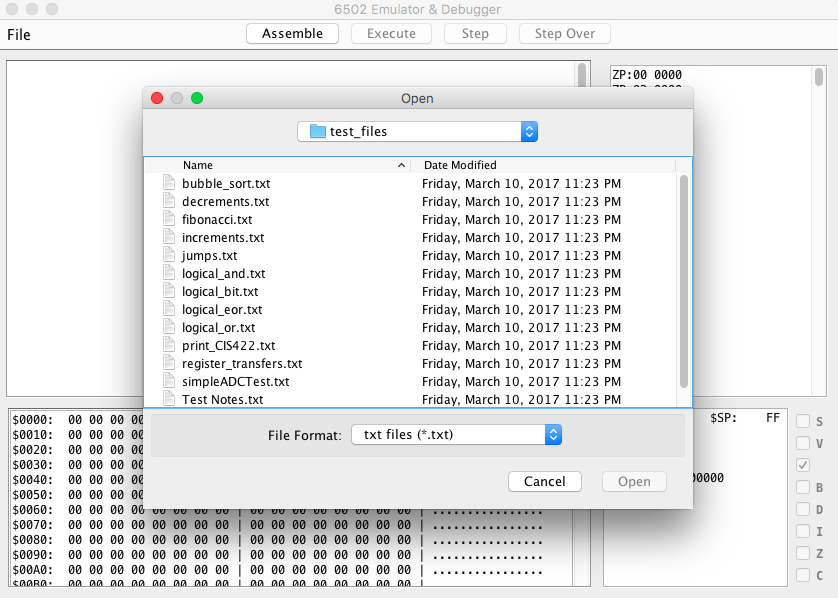
\includegraphics[width=9cm, height=6.4cm]{OpenFile}
		\caption{The Open Window}
	\end{figure}
	\clearpage
	\item \textbf{Find Text File to Import}\\
	Select the file that you would like to import in the Open window. Be sure that the file selected is a .txt file or else you will not be able to open the file. Select the file and press Open.
	\begin{figure}[h!]
		\centering
		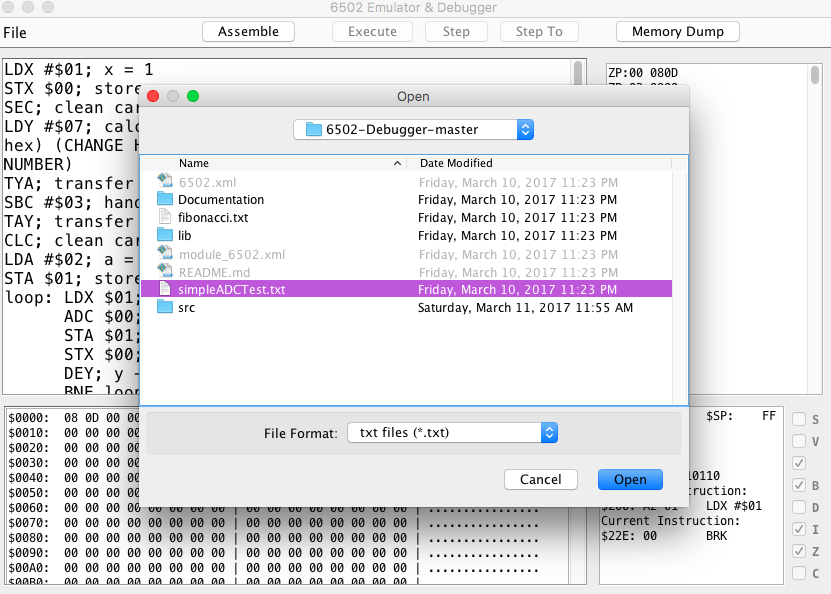
\includegraphics[width=9cm, height=6.4cm]{SelectFile}
		\caption{The Open Window}
	\end{figure}
	\par
	After this step, you will be left with the Main page of the 6502 Debugger with your code loaded in the main text window. 
	\begin{figure}[h!]
		\centering
		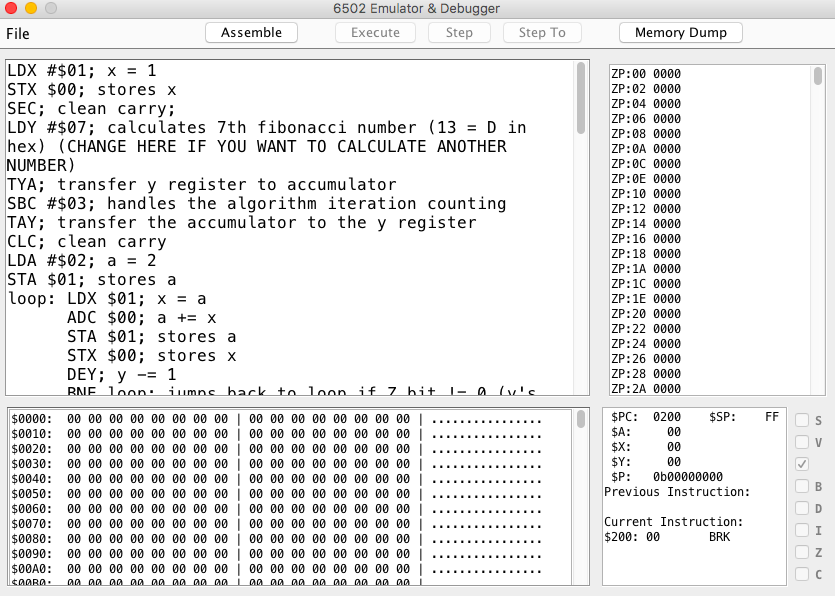
\includegraphics[width=9cm, height=6.4cm]{FibCode}
		\caption{Main Page with code loaded in the main text window}
	\end{figure}	
\end{enumerate}
\clearpage

\section{Assemble your Code}
\subsection{Overview}
Assembling your code can be done with a click of a button using this Debugger. 
\begin{enumerate}
	\item \textbf{Begin at the Main Page with Assembly Code loaded in the Main Window}\\
	To assemble code, you must have code loaded in the main window. This can be done by importing the code from a .txt file, copy and pasting the code, or typing it directly into the text window. 
	\item \textbf{Click the Assemble Button}\\
	The Assemble button is located in the centre of the task bar at the top of the window. 
	\par
	After this step, the first line of code should be highlighted green with the appropriate flags selected. 
	\begin{figure}[h!]
		\centering
		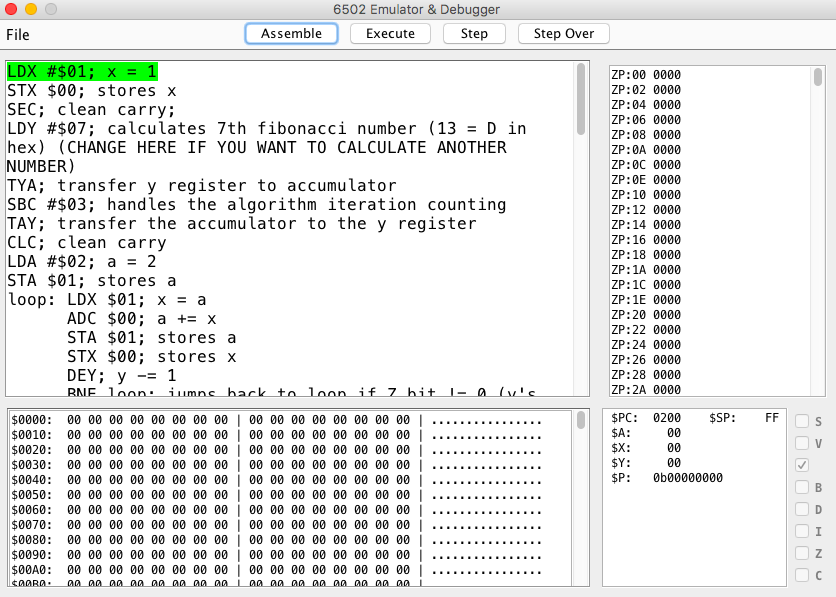
\includegraphics[width=8cm, height=5.74cm]{Assemble}
		\caption{The First Line of Code is Highlighted Green}
	\end{figure} 
\end{enumerate}

\section{Execute your Code}
\subsection{Overview}
Executing your loaded assembly code is easily done in the 6502 Debugger. 
\subsection{Procedure}
\begin{enumerate}
	\item \textbf{Begin by Assembling your Code}
	If needed, see "Assemble your Code" section for further instruction.
	\item \textbf{Click the Execute Button}
	The Execute button is located in the centre of the task bar at the top of the window.	
\end{enumerate}

\section{Using the "Step" Function}
\subsection{Overview}
To execute your code line by line, you can use the Debugger's Step function by simply clicking. 
\subsection{Procedure}
\begin{enumerate}
	\item \textbf{Begin by Assembling your Code}\\
	If needed, see "Assemble your Code" section for further instruction.
	\item \textbf{Click the Step Button}\\
	The Step button is located in the centre of the task bar at the top of the window.
	\par
	After this step, the current line of code highlighted in green will execute and the highlighting will move to the next line. 
	\begin{figure}[h!]
		\centering
		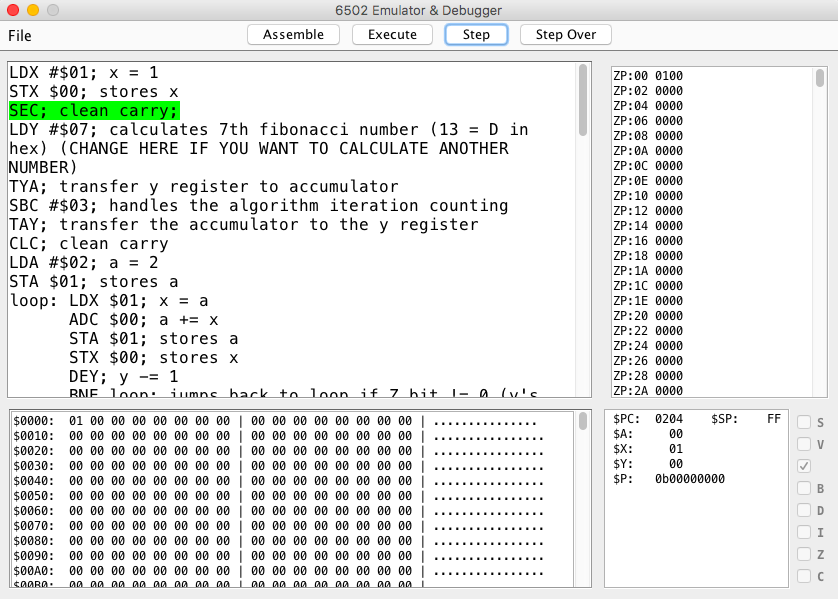
\includegraphics[width=8cm, height=5.74cm]{Execute}
		\caption{The Line Highlighted will Change}
	\end{figure}
\end{enumerate}
\clearpage

\section{Using the "Step to" Function}
\subsection{Overview}
The Step To function will allow you to skip to a function of your choosing. 
\subsection{Procedure}
\begin{enumerate}
	\item \textbf{Begin by Assembling your Code}\\
	If needed, see "Assemble your Code" section for further instruction.
	\item \textbf{Click the Step To Button}\\
	The Step To button is located in the centre of the task bar at the top of the window. If your Assembly Code does not have any defined functions, it will display an error.
	\begin{figure}[h!]
		\centering
		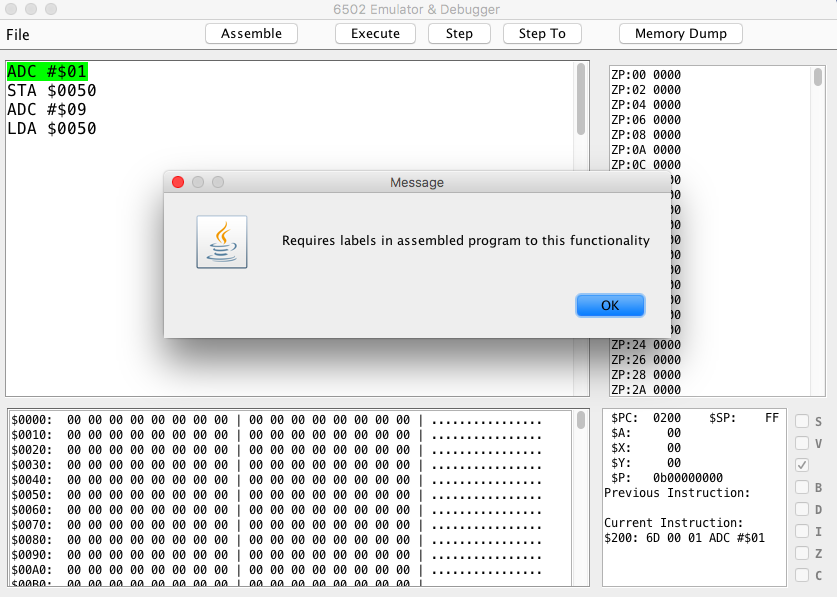
\includegraphics[width=8cm, height=5.74cm]{FailedStepTo}
		\caption{Unable to Perform the Step To Function}
	\end{figure}
	\par
	Otherwise, the Step To window will appear .
	\begin{figure}[h!]
		\centering
		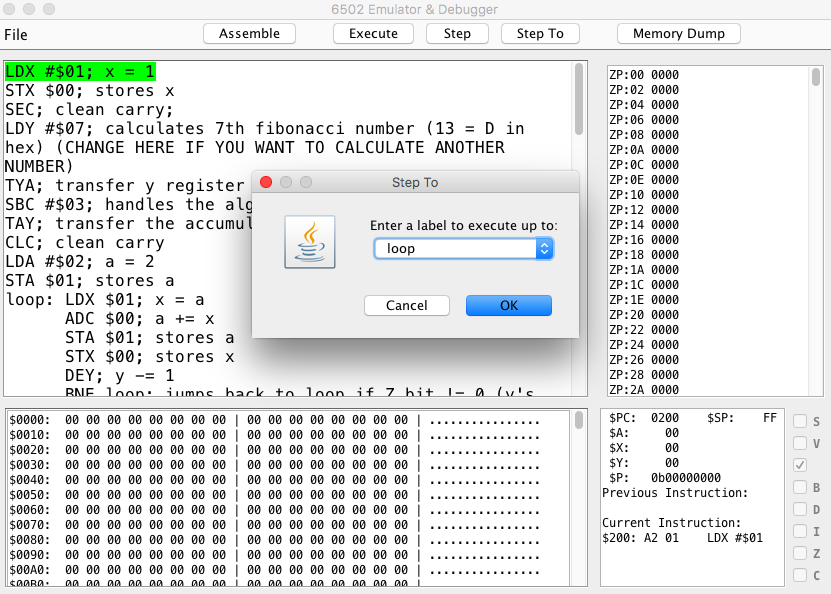
\includegraphics[width=8cm, height=5.74cm]{StepToClosedMenu}
		\caption{The Step To Window}		
	\end{figure} 
	\item \textbf{Select the Function to Step To}\\
	If you have multiple functions, open the drop down menu in the Step To window, select your chosen function, and click OK. 
	\begin{figure}[h!]
		\centering
		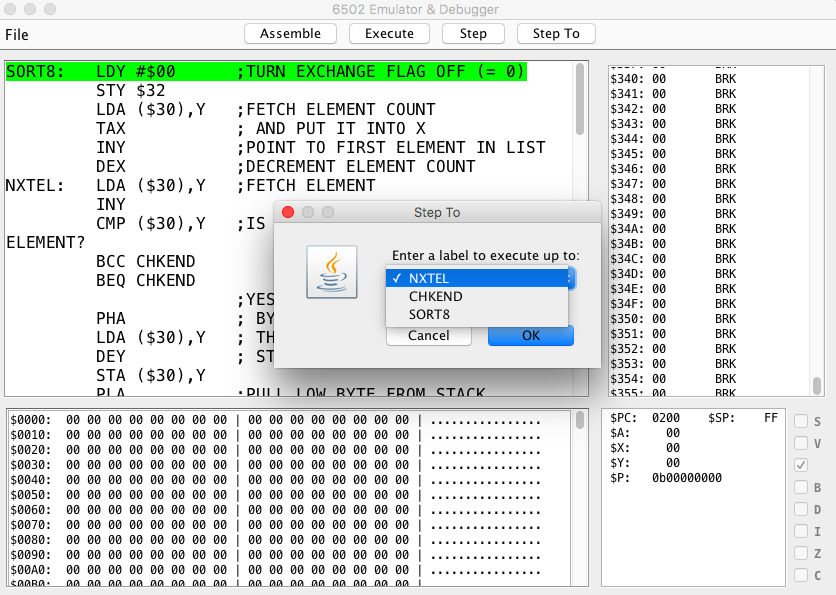
\includegraphics[width=8cm, height=5.74cm]{StepToOpenMenu}
		\caption{The Open Drop Down Menu in the Step To Window}
	\end{figure}
	\par
	After this step, your chosen function will be highlighted in green. 
	\begin{figure}[h!]
		\centering
		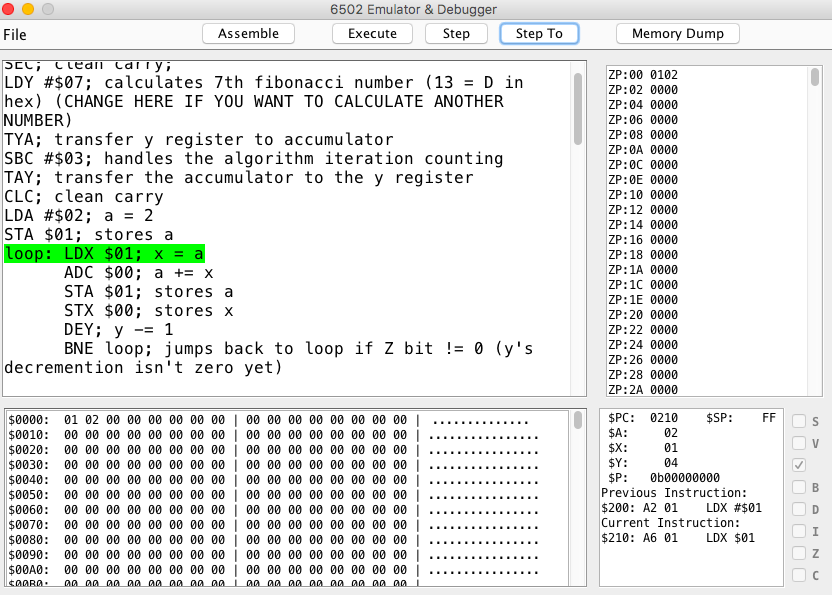
\includegraphics[width=8cm, height=5.74cm]{AfterStepTo}
		\caption{After Step To has been executed}
	\end{figure}
\end{enumerate}
\clearpage

\section{Save an Existing Program}
\subsection{Overview}
\begin{enumerate}
	\item \textbf{Click Save in the drop down File Menu}
	You will see the File menu on the top left-hand corner of the window. Click File so the drop down menu appears and click Save, a new window will appear. 
	\begin{figure}[h!]
		\centering
		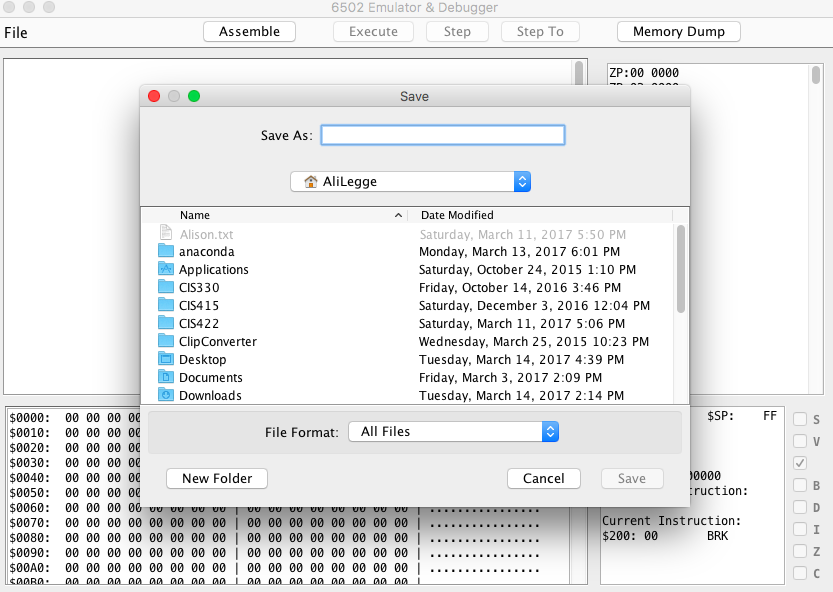
\includegraphics[width=8cm, height=5.74cm]{Save}
		\caption{After the Save Window Opens}
	\end{figure}
	\item \textbf{Save the File}
	Type the filename and click Save.
	\begin{figure}[h!]
		\centering
		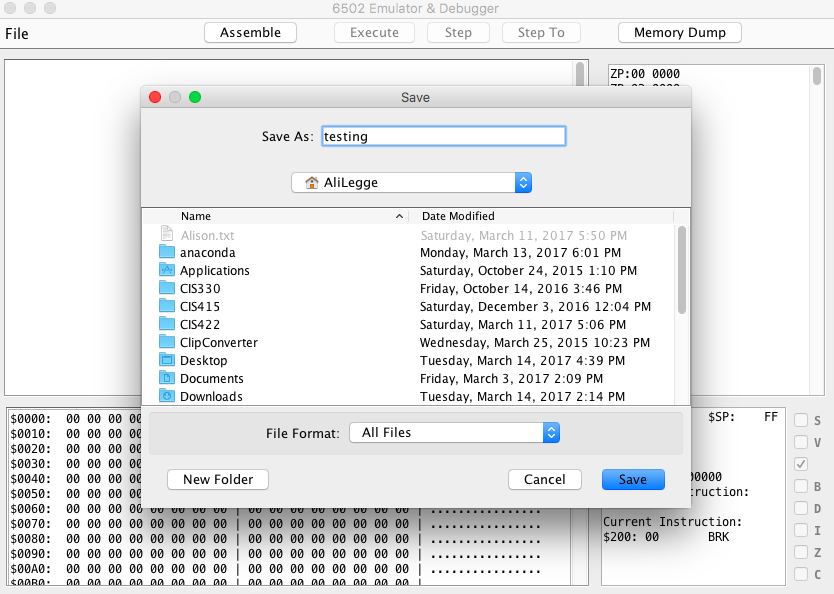
\includegraphics[width=8cm, height=5.74cm]{SaveText}
		\caption{After the Name has been Typed}
	\end{figure}
\end{enumerate}


\end{document}